\chapter{Design of the control system} \label{ch4}

In the previous chapters, we outlined deep reinforcement learning fundamentals and the most critical underlying concepts, and then we discussed the choice made about the technologies to use as baselines for our experiments. The decision fell on Anki Cozmo because of the high-quality SDK provided to developers and the versatility and flexibility provided by PyTorch, especially in a research context.

The next step in this thesis is the merge of reinforcement learning theory with the tool presented previously. Indeed, this chapter aims to describe this merge process that results in the design of the control system for reinforcement learning experiments with Anki Cozmo. The work presented in this section represents one of the contributions of our thesis and the necessary step to start reinforcement learning experiments.

The outline of the whole ecosystem with the description of interfaces, frameworks and technologies used occupies the first section of the chapter. This part also comprehends a discussion about DDPG \cite{lillicrap2015continuous} and SAC \cite{haarnoja2018soft, haarnoja2018alg} implementation with references to the choice made in terms of hyper-parameters and problems faced.

The second part of the chapter aims to describe the implementation of Anki Cozmo OpenAI Gym environment from the problem formalisation as MDP to the implementation of human-robot interaction.

In the final section of this chapter, the design and setup of the real track will be discussed together with a discussion about the problems faced and the choice made to overcome them.

\section{Outline of the system}

The development of the control system for Anki Cozmo was the main contribution of the thesis, together with the implementation of DDPG and SAC algorithm. The main aim of this work was to create an OpenAI Gym environment capable of interacting with a robot in the real world, not just through the usage of a simulator. OpenAI Gym usually provides plain and straightforward interfaces to interact with simulated environments: we decided to exploit these functions to allow the application of reinforcement learning algorithm directly in the real-world decision of the robot.

The fundamental source of inspiration to develop this control system was \cite{kendall2018learning,kendall2019learning}. This publication represents, as its authors reported,  the first reinforcement learning self-driving experiment where a car learned to drive through the application of a reinforcement learning algorithm, by trial and error. They first trained the model exploiting Deep Deterministic Policy Gradient (DDPG) in a simulator for many epochs and, after this learning process, they managed to transfer the knowledge acquired in the simulator in real-world experiments. 

We decided to export and implement these ideas in our project, adapting them to the specificities and particularities of the Cozmo setup. The resulting system can be summed up by \vref{fig:system} which provide a schematic overview of every technology employed and the interaction among them.
This section aims to describe as clearly as possible all the components of the control system we designed.

\tikzset{every picture/.style={line width=0.75pt}} %set default line width to 0.75pt        

\begin{figure}
	\tikzset{every picture/.style={line width=0.75pt}} %set default line width to 0.75pt    
	\centering
	\scalebox{0.85}{


		\tikzset{every picture/.style={line width=0.75pt}} %set default line width to 0.75pt        

	\begin{tikzpicture}[x=0.75pt,y=0.75pt,yscale=-1,xscale=1]
		%uncomment if require: \path (0,438); %set diagram left start at 0, and has height of 438

		%Image [id:dp06991158821872456] 
		\draw (239.75,55) node  {
\includegraphics[width=115.13pt,height=52.5pt]{img/python.png}};
		%Image [id:dp3729269645681633] 
		\draw (240.25,198.5) node  {
\includegraphics[width=46.88pt,height=50.25pt]{img/gym.png}};
		%Image [id:dp09149607927009118] 
		\draw (94.75,200.91) node  {
\includegraphics[width=124.13pt,height=25.37pt]{img/pytorch.png}};
		%Image [id:dp30806594376010465] 
		\draw (351.92,200) node  {
\includegraphics[width=40.38pt,height=52.5pt]{img/flask.png}};
		%Straight Lines [id:da3933293266418665] 
		\draw    (239.98,93) -- (239.52,159) ;
		\draw [shift={(239.5,162)}, rotate = 270.4] [fill={rgb, 255:red, 0; green, 0; blue, 0 }  ][line width=0.08]  [draw opacity=0] (8.93,-4.29) -- (0,0) -- (8.93,4.29) -- cycle    ;
		\draw [shift={(240,90)}, rotate = 90.4] [fill={rgb, 255:red, 0; green, 0; blue, 0 }  ][line width=0.08]  [draw opacity=0] (8.93,-4.29) -- (0,0) -- (8.93,4.29) -- cycle    ;
		%Straight Lines [id:da24057878811893751] 
		\draw    (167.75,200.25) -- (203.75,200.25) ;
		\draw [shift={(206.75,200.25)}, rotate = 180] [fill={rgb, 255:red, 0; green, 0; blue, 0 }  ][line width=0.08]  [draw opacity=0] (8.93,-4.29) -- (0,0) -- (8.93,4.29) -- cycle    ;
		\draw [shift={(164.75,200.25)}, rotate = 0] [fill={rgb, 255:red, 0; green, 0; blue, 0 }  ][line width=0.08]  [draw opacity=0] (8.93,-4.29) -- (0,0) -- (8.93,4.29) -- cycle    ;
		%Straight Lines [id:da10061083103025648] 
		\draw    (283.75,199.58) -- (318.5,199.58) ;
		\draw [shift={(321.5,199.58)}, rotate = 180] [fill={rgb, 255:red, 0; green, 0; blue, 0 }  ][line width=0.08]  [draw opacity=0] (8.93,-4.29) -- (0,0) -- (8.93,4.29) -- cycle    ;
		\draw [shift={(280.75,199.58)}, rotate = 0] [fill={rgb, 255:red, 0; green, 0; blue, 0 }  ][line width=0.08]  [draw opacity=0] (8.93,-4.29) -- (0,0) -- (8.93,4.29) -- cycle    ;
		%Image [id:dp8556439958741602] 
		\draw (567,186) node  {
\includegraphics[width=52.5pt,height=52.5pt]{img/user.png}};
		%Straight Lines [id:da26821981951432505] 
		\draw    (385.5,184.58) -- (499.5,184.58) ;
		\draw [shift={(502.5,184.58)}, rotate = 180] [fill={rgb, 255:red, 0; green, 0; blue, 0 }  ][line width=0.08]  [draw opacity=0] (8.93,-4.29) -- (0,0) -- (8.93,4.29) -- cycle    ;

		%Straight Lines [id:da7643998387312995] 
		\draw    (388.5,214.58) -- (412.5,214.58) -- (500.5,214.58) ;

		\draw [shift={(385.5,214.58)}, rotate = 0] [fill={rgb, 255:red, 0; green, 0; blue, 0 }  ][line width=0.08]  [draw opacity=0] (8.93,-4.29) -- (0,0) -- (8.93,4.29) -- cycle    ;
		%Straight Lines [id:da5051570254396728] 
		\draw    (240.5,256) -- (240.5,278) ;
		\draw [shift={(240.5,281)}, rotate = 270] [fill={rgb, 255:red, 0; green, 0; blue, 0 }  ][line width=0.08]  [draw opacity=0] (8.93,-4.29) -- (0,0) -- (8.93,4.29) -- cycle    ;
		\draw [shift={(240.5,253)}, rotate = 90] [fill={rgb, 255:red, 0; green, 0; blue, 0 }  ][line width=0.08]  [draw opacity=0] (8.93,-4.29) -- (0,0) -- (8.93,4.29) -- cycle    ;
		%Rounded Rect [id:dp9694318857670313] 
		\draw   (2,25.5) .. controls (2,15.28) and (10.28,7) .. (20.5,7) -- (464,7) .. controls (474.22,7) and (482.5,15.28) .. (482.5,25.5) -- (482.5,300.5) .. controls (482.5,310.72) and (474.22,319) .. (464,319) -- (20.5,319) .. controls (10.28,319) and (2,310.72) .. (2,300.5) -- cycle ;
		%Image [id:dp9562999520117128] 
		\draw (99,377) node  {
\includegraphics[width=52.5pt,height=52.5pt]{img/tablet.png}};
		%Straight Lines [id:da22030012036466173] 
		\draw    (98.5,295) -- (186.5,295) ;
		\draw [shift={(189.5,295)}, rotate = 180] [fill={rgb, 255:red, 0; green, 0; blue, 0 }  ][line width=0.08]  [draw opacity=0] (8.93,-4.29) -- (0,0) -- (8.93,4.29) -- cycle    ;

		%Straight Lines [id:da28839463654139263] 
		\draw    (98.5,295) -- (98.5,339) ;
		\draw [shift={(98.5,342)}, rotate = 270] [fill={rgb, 255:red, 0; green, 0; blue, 0 }  ][line width=0.08]  [draw opacity=0] (8.93,-4.29) -- (0,0) -- (8.93,4.29) -- cycle    ;

		%Straight Lines [id:da2120925552884272] 
		\draw  [dash pattern={on 0.84pt off 2.51pt}]  (154.75,380.58) -- (473.5,380.58) ;

		\draw [shift={(151.75,380.58)}, rotate = 0] [fill={rgb, 255:red, 0; green, 0; blue, 0 }  ][line width=0.08]  [draw opacity=0] (8.93,-4.29) -- (0,0) -- (8.93,4.29) -- cycle    ;
		%Image [id:dp7151280650926004] 
		\draw (535.32,366) node  {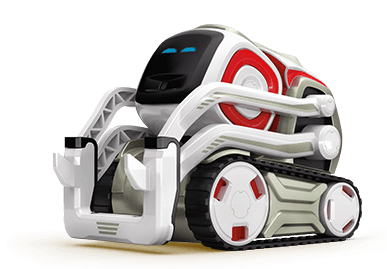
\includegraphics[width=96.27pt,height=69.12pt]{img/cozmo.png}};
		%Straight Lines [id:da948112813701837] 
		\draw  [dash pattern={on 0.84pt off 2.51pt}]  (151.75,402.58) -- (470.5,402.58) ;
		\draw [shift={(473.5,402.58)}, rotate = 180] [fill={rgb, 255:red, 0; green, 0; blue, 0 }  ][line width=0.08]  [draw opacity=0] (8.93,-4.29) -- (0,0) -- (8.93,4.29) -- cycle    ;

		%Image [id:dp8991970614844648] 
		\draw (332,113) node  {
\includegraphics[width=36pt,height=36pt]{img/tensorflow.png}};
		%Straight Lines [id:da8686562029937168] 
		\draw    (257.5,118) -- (297.5,118) ;
		\draw [shift={(300.5,118)}, rotate = 180] [fill={rgb, 255:red, 0; green, 0; blue, 0 }  ][line width=0.08]  [draw opacity=0] (8.93,-4.29) -- (0,0) -- (8.93,4.29) -- cycle    ;

		%Straight Lines [id:da7903500333471788] 
		\draw    (257.5,118) -- (257.5,165) ;


		%Straight Lines [id:da017309376357115047] 
		\draw    (557.15,117.91) -- (557.15,93) ;
		\draw [shift={(557.15,90)}, rotate = 450] [fill={rgb, 255:red, 0; green, 0; blue, 0 }  ][line width=0.08]  [draw opacity=0] (8.93,-4.29) -- (0,0) -- (8.93,4.29) -- cycle    ;

		%Straight Lines [id:da46777924457369235] 
		\draw    (557.15,117.91) -- (453.67,117.91) ;


		%Image [id:dp9871015067821471] 
		\draw (559,44) node  {
\includegraphics[width=42pt,height=42pt]{img/analysis.png}};

		% Text Node
		\draw (569,227) node  [font=\footnotesize] [align=left] {Human-Robot Interaction};
		% Text Node
		\draw (435,175) node  [font=\footnotesize] [align=left] {Image};
		% Text Node
		\draw (436,204) node  [font=\footnotesize] [align=left] {Commands};
		% Text Node
		\draw (114,22) node   [align=left] {\textbf{Development Machine}};
		% Text Node
		\draw    (196.5,282.5) -- (287.5,282.5) -- (287.5,307.5) -- (196.5,307.5) -- cycle  ;
		\draw (242,295) node   [align=left] {Cozmo SDK};
		% Text Node
		\draw (100,423) node   [align=left] {\textbf{Android Device}};
		% Text Node
		\draw (120,276) node   [align=left] {{\footnotesize ADB}};
		% Text Node
		\draw (323,420) node   [align=left] {Wi-Fi Connection};
		% Text Node
		\draw (536,420) node   [align=left] {\textbf{Cozmo}};
		% Text Node
		\draw (319,370) node  [font=\footnotesize] [align=left] {Image};
		% Text Node
		\draw (320,394) node  [font=\footnotesize] [align=left] {Commands};
		% Text Node
		\draw (396,119) node   [align=left] {TensorBoard};
		% Text Node
		\draw (559,75) node  [font=\footnotesize,] [align=left] {Data Analysis};
		% Text Node
		\draw (241,242) node   [align=left] {OpenAI Gym};


	\end{tikzpicture}
	}
	\caption[Interaction Human/Robot]{Interaction between the user and Anki Cozmo. The main Python script utilises OpenAI Gym for the reinforcement learning component and PyTorch for the deep learning one. The user can interact with the flow of the system through a simple web app implemented using HTML, CSS, JS that communicates with a Flask backend. This component interacts directly with OpenAI Gym and the Cozmo SDK to provide information for the user (e.g.\ images, learning information) and the robot (e.g.\ commands). The last component consists in TensorBoard thanks to the script can store results that can be retrieved later by the user.}
	\label{fig:system}
\end{figure}

\subsection{Human-Robot Interaction}

It is noticeable that the simulator can undoubtedly be programmed to understand when the car is outside the track. In a reinforcement learning scenario, this fact facilitates the restarting procedure for an episode: the developer has to bind some events or actions to a process that stops the current episode, put the car on the road again and starts the next experiment. In the real world, the situation is more complicated because there are more variables to take into account: the most critical factor is that the failure of an episode in the simulator has no threats or costs, while real-world experiments failures could lead to high costs. Despite this point, the application of such experiment typology in a real environment instead of a mere simulation represents an exciting challenge that could bring reinforcement learning to the next level. In order to make experiments as safe as possible, the authors of \cite{kendall2018learning,kendall2019learning} implemented a self-driving system designed explicitly for reinforcement learning experiments where the car driver has the faculty of stopping the car when it is going to run off the road or in a dangerous situation and relocating it in the nearest safe position to start the next learning episode.

For this reason, we firstly implemented a straightforward interface using a web app implemented using plain HTML, CSS and Javascript for the frontend and Flask as backend. The aim of this application is allowing user interaction with Cozmo and Flask represented the right choice to allow the communication between this interface and the OpenAI Gym environment. The user can see a sort of live streaming from the camera of Cozmo directly in the web app and can send commands to the robot through the computer keyboard. Just as example

In this context, the human-robot interaction has a crucial role in the learning process because it is the source of all improvements and flaws of the learning process: the robot learns which actions are worthy and which are not, but the human is the one who decides the correctness of each action, carrying its unconscious bias in the algorithm. We will discuss the experiments and their results thoroughly in \vref{ch5,ch6}.




% \todomacaluso{
% 	\begin{itemize}
% 		\item Introduction to the chapter
% 		\item General description of the control systems with a diagram representing all the technologies involved.
% 		\item Setup of the algorithms (DDPG, SAC)
% 		      \begin{itemize}
% 			      \item We decided to rewrite both algorithms without using libraries directly. The first motivation was didactical, implementing from scratch is helpful to understand the practical implementation of the algorithm better, but also to make it possible to implement the singularity of the real Cozmo environment.
% 			      \item The interaction with OpenAI Gym and PyTorch
% 			      \item Discussion about Hyper-Parameters and the problems faced in the real world situation in the selection of these parameters.
% 		      \end{itemize}
% 		\item Setup and implementation of CozmoEnv
% 		      \begin{itemize}
% 			      \item Technologies used to implement the interaction between the Cozmo SDK and OpenAI Gym.
% 			      \item Differences from the simulated environment caused by the need for direct human interaction.
% 			      \item Implementation of human interaction in the system.
% 		      \end{itemize}
% 		\item Setup of the real Environment
% 		      \begin{itemize}
% 			      \item The Track design
% 			      \item Analysis of the problems:
% 			            \begin{itemize}
% 				            \item Reflection
% 				            \item Background and Horizon
% 			            \end{itemize}
% 			      \item (Single Line Track)
% 		      \end{itemize}
% 	\end{itemize}
% }

% \section{The track}

% The design and training of a good driving model cannot go beyond the construction and design of the road. For this reason, some time was spent searching the better way to build a path where to train Cozmo.
% This section aims to present the central concept and decisions made about the design of the track for the experiments, starting from the materials used, up to the description of the dimensional choices applied.

% \subsection{Track requirements}

% It is essential to explain the primary needs of the road before proceeding with the description of the choices made.

% Firstly, the track needs to be easily transportable to allow various attempt with different locations and environmental conditions that could affect the training phase. In particular, it is necessary to use a material less reflective as possible to avoid problems during the learning process.
% Another crucial factor is the dimension of the lane, which must reproduce an environment similar to the real one. It can be done analyzing the ratio of the size of a vehicle to the width of a road. On average, a family car is about $160$-$170$cm large, while a lane width can vary between $275$cm and $375$cm. Cozmo width is about $5.5$cm, which results in a ratio of $1/30$. Therefore, the scaled lane must be between $9$cm and $12.5$cm.

% \subsection{Track design and materials}

% The first choice to make is the one about the type of material to use as terrain for the track. The first choice was the black floor of the Data Science laboratory of Eurecom. It was useful only during the initial design and development of the control system to build small pieces of track in which testing functionalities. This solution had numerous drawbacks such as the impracticality to transport and high light reflection. 

% The following list provides a brief report of the various solutions taken into account during the thesis, together with an analysis of advantages and drawbacks.

% \begin{itemize}
% 	\item \textit{Covering fabric}: this material is easily transportable, but it has a high light reflection, and its structure is prone to make wrinkles and dunes challenging to remove.
% 	\item \textit{Tar paper}: this solution slightly diminished the reflection problem compared to the previous choice, but the material was fragile and with the same drawbacks of the covering fabric.
% 	\item \textit{Cotton fabric}: this solution offers an easily  transportable material with reduced light reflection where it is easy to remove wrinkles and dunes.
% \end{itemize}

% Summing up, it is noticeable from this analysis that the cotton fabric provides the right trade-off among all requirements reported before.

% The structure of the road is also composed by the lane. The implementation of this part was done using a simple paper tape of width equal to $2.5$cm. As described in the beginning of this section, the width of the lane must be between $9$cm and $12.5$cm to provide a context similar to the real one. Because of the narrow and limited angle of vision provided by Cozmo camera, $10$cm-width was set: positioning the tape with a distance greater than $10$cm would result in a great part of the tape outside the view of the camera.